\PassOptionsToPackage{table, xcdraw, dvipsnames}{xcolor}

% \documentclass[11pt, presentation]{beamer}
\documentclass[11pt, handout]{beamer}
\usetheme{yeast}

\usepackage{lipsum}
\usepackage{tabularx}
\renewcommand{\arraystretch}{2}
\renewcommand\tabularxcolumn[1]{m{#1}}

\usepackage{appendixnumberbeamer}
\setbeamertemplate{frametitle continuation}{}

\newcommand \albf[1]{\textbf{\alert{#1}}}

% defs
\def\cmd#1{\texttt{\color{red}\footnotesize $\backslash$#1}}
\def\env#1{\texttt{\color{blue}\footnotesize #1}}
\definecolor{db}{rgb}{0,0,0.5}
\definecolor{dr}{rgb}{0.6,0,0}
\definecolor{dg}{rgb}{0,0.5,0}
\definecolor{halfgray}{gray}{0.55}
\definecolor{hl}{HTML}{fafe7b}

\newcommand<>\hlbox[2]{%
  \alt#3{\makebox[\dimexpr\width-1\fboxsep]{\colorbox{#1}{#2}}}{#2}%
}

% Allow for overlay of cellcolor function
\renewcommand<>\cellcolor[1]{\only#2{\beameroriginal\cellcolor{#1}}}
\renewcommand<>\rowcolor[1]{\only#2{\beameroriginal\rowcolor{#1}}}

\usepackage{xspace}
\newcommand{\pan}{\textsc{PAn}\xspace}
\newcommand{\paic}{\textsc{PAic}\xspace}
\newcommand{\pata}{\textsc{PAta}\xspace}
\newcommand{\ata}{\textsc{Ata}\xspace}
\newcommand{\psed}{\textsc{PSed}\xspace}
\newcommand{\sed}{\textsc{Sed}\xspace}
\newcommand{\psedf}{Proto-Seediq\xspace}
\newcommand{\stg}{\textsc{Tg}\xspace}
\newcommand{\stgf}{Tgdaya\xspace}
\newcommand{\ptotr}{\textsc{PToTr}\xspace}
\newcommand{\ptotrf}{Proto-Toda-Truku\xspace}
\newcommand{\scto}{\textsc{CTo}\xspace}
\newcommand{\sctof}{Central Toda\xspace}
\newcommand{\seto}{\textsc{ETo}\xspace}
\newcommand{\setof}{Eastern Toda\xspace}
\newcommand{\ptr}{\textsc{PTr}\xspace}
\newcommand{\sctr}{\textsc{CTr}\xspace}
\newcommand{\sctrf}{Central Truku\xspace}
\newcommand{\setr}{\textsc{ETr}\xspace}
\newcommand{\setrf}{Eastern Truku\xspace}

\addbibresource{../ref.bib}

% \setbeamertemplate{headline}[progress bar]

% 自訂指令 %
\newcommand{\shb}[1]{\textsuperscript{#1}}
\newcommand{\xb}[1]{\textsubscript{#1}}
\newcommand{\aikai}[1]{\textcolor{red}{\textbf{#1}}}
\newcommand{\cvc}{$\symbb{CVC}$\xspace}


\title[The Historical Development of the Seediq Language]{\textbf{The Historical Development of\\the Seediq Language}\\\large{~}\\\large{\textit{Eluw Ndaan Kari Seediq\\賽德克語的歷史發展}}}
\author[W. Song]{Walis Hian-chi Song\\宋硯之}
\institute[NTHU]{}
\date{Feb 25, 2025}

\begin{document}

\maketitle

\begin{frame}{Outline}
  \tableofcontents
\end{frame}

\section{Introduction}

\begin{frame}{Abbreviations}
    \begin{itemize}
        \item Proto-languages
        \begin{itemize}
        \item \paic = Proto-Atayalic
        \item \pan = Proto-Austronesian
        \item \pata = Proto-Atayal
        \item \psed = \psedf
        \end{itemize}
    \end{itemize}
        \begin{itemize}
        \item Seediq dialects
        \begin{itemize}
            \item \scto = \sctof
            \item \sctr = \sctrf
            \item \seto = \setof
            \item \setr = \setrf
            \item \stg = \stgf
        \end{itemize}
    \end{itemize}
\end{frame}

\begin{frame}{Basic introduction - 1}
    \begin{itemize}
        \item<1-> Seediq is an Austronesian language spoken in Central and Eastern mountainous area of Taiwan. 
        \item<2-> Together with Atayal, they form an Atayalic subgroup, which is considered to be a primary branch of Austronesian family (\cite{blust1999subgrouping}). 
        \item<3-> Five dialects will be included in this thesis: Tgdaya (德固達雅), Central Toda (都達), Eastern Toda (陶賽), Central Truku (德鹿谷) and Eastern Truku (太魯閣).
    \end{itemize}
\end{frame}

\begin{frame}{Basic introduction - 2}
    \begin{figure}
        \centering
        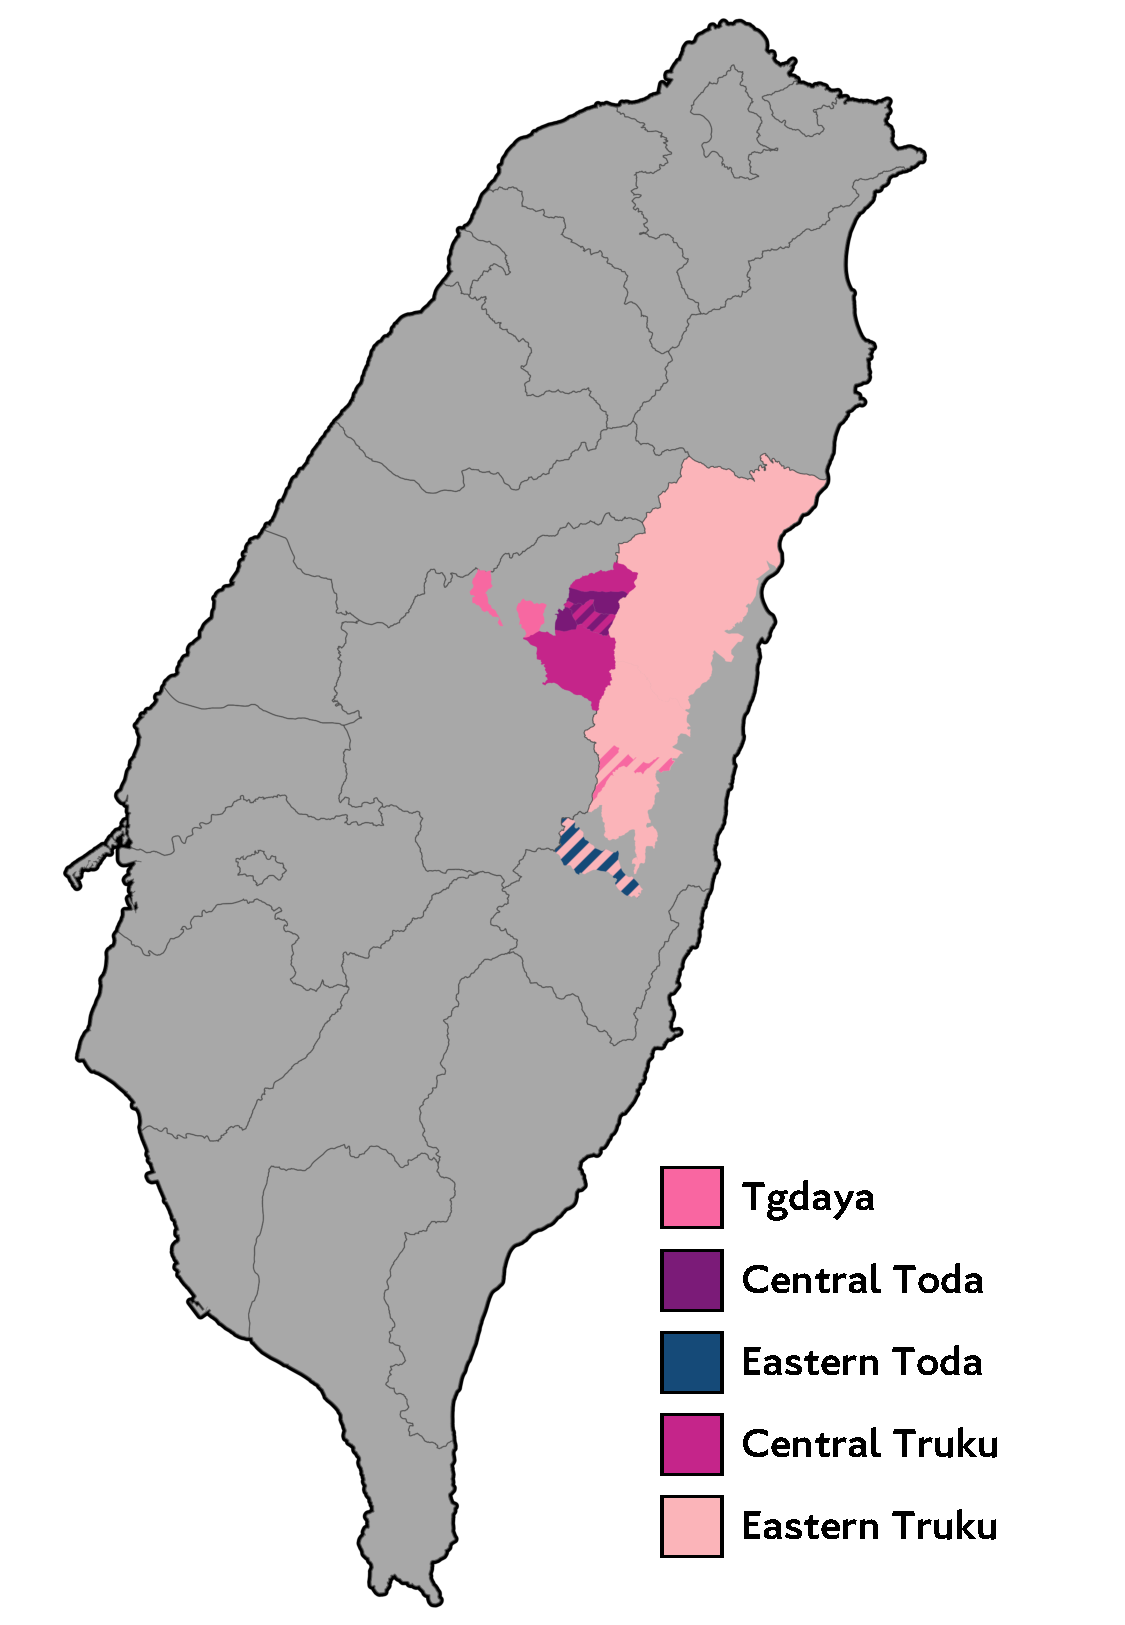
\includegraphics[height=0.9\textheight]{../img/dialectmap.pdf}
    \end{figure}
\end{frame}

\begin{frame}{Methodology - 1}{The Comparative Method}
\begin{itemize}
    \item<1-> This thesis employs the Comparative Method in historical linguistics to reconstruct Proto-Seediq and classify Seediq dialects, following essential steps (\cite{fox1995linguistic}).
    \item<2-> \albf{Step 1:} Collecting words and identify cognates among Seediq dialects, while ruling out thoses with chance, universals, and borrowing as explanations.
    \begin{itemize}
        \item<3-> \albf{Cognates:} words in basic vocabulary that are similar or same in both form and meaning, showing regular sound correspondences.
    \end{itemize}
    \item<4-> \albf{Step 2:} Setting up sound correspondences and group the correspondence sets together based on phonetic similarity.
\end{itemize}
\end{frame}

\begin{frame}{Methodology - 2}{The Comparative Method}
\begin{itemize}
    \item<1-> \albf{Step 3:} Reconstructing the protophonemes and assign their phonetic values.
    \begin{itemize}
        \item<2-> sound change should be plausible and natural in language developments, and regular
        \item<3-> a reconstructed phoneme should minimize changes in both place and manner of articulation
    \end{itemize}
    \item<4-> \albf{Step 4:} Reconstructing the lexicon based on the sound correspondences and protophonemes.
\end{itemize}
\end{frame}

\begin{frame}{Methodology - 3}{The Comparative Method}
\begin{itemize}
    \item<1-> \albf{Step 5:} Determining a subgrouping of the Seediq language.
    \begin{itemize}
        \item<2-> based on shared innovations, not retentions
        \item<3-> sporadic/rare SCs are better than common ones
        \item<4-> ``drift'' --- common sound changes occurring individually in closely related languages/dialects --- must be ruled out
        \item<5-> \albf{Phonological evidence:} Mergers, conditioned shifts/splits, etc.
        \item<6-> \albf{Lexical evidence:} Shared lexical innovations (including exclusive ``word-modifications'' such as affixing, partial replacements on words. See the discussion of ``Special doublet phenomenon'')
    \end{itemize}
\end{itemize}
\end{frame}

\begin{frame}{Methodology - 4}{Top-down reconstruction method}
    \begin{itemize}
        \item<1-> Is also called ``inverted reconstruction'' (\cites[512--16]{hockett1958course}[346]{anttila1972introduction})
        \item<2-> If there is a relevant reconstruction in language X's ancestral language(s) based on other languages, we can use those forms to reconstruct the form's in X \albf{from above} (\cite[88]{fox1995linguistic}).
        \item<3-> Details and practical implementation will be introduced later.
    \end{itemize}
\end{frame}

\begin{frame}{Data sources}
\begin{itemize}
    \item \stg: \textcite{ILRDFEdict,ILRDF1000words,Seddatabase,watandiro2009seddict} + Fieldwork
    \item \scto: \textcite{ILRDF1000words,Seddatabase,watandiro2009seddict} + Fieldwork
    \item \seto: \textcite{lee2015tawsa}
    \item \sctr: \textcite{ILRDF1000words,Seddatabase,watandiro2009seddict}
    \item \setr: \textcite{ILRDFEdict,ILRDF1000words}
\end{itemize}
\end{frame}

\begin{frame}{Orthographic conventions}
    \begin{table}[]
    \centering
    \resizebox{0.9\textwidth}{!}{%
    \begin{tabular}{l|ccccccc}
    \textbf{This thesis} & c     & ɟ & h   & ŋ   & r   & l          & y   \\ \hline
    \textbf{CIP/MOE}    & c     & j & h   & ng  & r   & l          & y   \\
    \textbf{IPA}        & [ts\~{}tɕ] & [ɟ\~{}dʑ]  & [ħ] & [ŋ] & [ɾ] & [l\~{}ɮ] & [j]
    \end{tabular}%
    }
    \end{table}
    \begin{itemize}
        \item {<}r> has some other variants, such as [ɾ], [ɻ], [ɺ], [r], etc. The pronunciation depends on dialect or idiolect.
        \item Here I only listed those symbol that different from IPA. 
    \end{itemize}
\end{frame}

\section{Proto-Seediq Phonology}

\begin{frame}{Consonants}
    \begin{table}[]
\centering
\resizebox{\textwidth}{!}{%
\begin{tabular}{l|cc|cc|cc|cc|cc|cc}
                    & \multicolumn{2}{c|}{Bilabial} & \multicolumn{2}{c|}{Dental/Alveolar} & \multicolumn{2}{c|}{Palatal} & \multicolumn{2}{c|}{Velar} & \multicolumn{2}{c|}{Uvular} & \multicolumn{2}{c}{Pharyngeal} \\ \hline
Stop                & *p            & *b           & *t               & *d               &             &               & *k          &             & *q            &            &                 &              \\
Affricate           &               &              & *c               &                  &             &               &             &             &               &            &                 &              \\
Fricative           &               &              & *s               &                  &             &               & *x          & *g          &               &            & *h              &              \\
Nasal               &               & *m           &                  & *n               &             &               &             & *ŋ          &               &            &                 &              \\
Lateral  &               &              &                  & *l               &             &               &             &             &               &            &                 &              \\
Tap                 &               &              &                  & *r               &             &               &             &             &               &            &                 &              \\
Glide               &               & *w           &                  &                  &             & *y            &             &             &               &            &                 &             
\end{tabular}%
}
\end{table}
\end{frame}

\begin{frame}{Vowels}
\begin{table}[]
\centering
\resizebox{0.6\textwidth}{!}{%
\begin{tabular}{c|ccc}
     & Front & Central & Back \\ \hline
High & *i    &         & *u   \\
Mid  &       & *ə      &      \\
Low  &       & *a      &     
\end{tabular}%
}
\end{table}

\begin{center}
``diphthongs'' (VG sequences): *aw, *ay and *uy.
\end{center}
\end{frame}


\begin{frame}{Phonotactics}
\begin{itemize}
    \item Stress: penultimate
    \item Word-final *-p, *-b, *-d, *-c, *-m, *-ag are not allowed
    \item Only one word starts with an *x-, which is *xiluy `iron'
\end{itemize}
\end{frame}

\begin{frame}{Syllable types}
\renewcommand\arraystretch{1.5}
\begin{table}[!htbp]
\centering
\resizebox{\textwidth}{!}{%
\begin{tabular}{lllllll}
\hline
     & \multicolumn{2}{l}{Prepenultimate} & \multicolumn{2}{l}{Penultimate} & \multicolumn{2}{l}{Final}        \\ \hline
V             & ---               &                & *\textbf{i}.ma        & `who'            & *sə.kə.lu.\textbf{i} & `startled'         \\
VC            & ---               &                & ---          &                  & *sa.\textbf{un}      & `to go (\acs{pv})'   \\
CV            & *\textbf{qə}.si.ya         & `water'        & *qə.\textbf{si}.ya    & `water'          & *qə.si.\textbf{ya}   & `water'            \\
VG            & ---               &                & *\textbf{aw}.raw      & `k.o. bamboo'    & *də.mu.\textbf{uy}   & `to hold (\acs{av})' \\
CVC           & ---               &                & ---          &                  & *ba.\textbf{raq}     & `lungs'            \\
CVG           & ---               &                & *\textbf{daw}.riq     & `eye'            & *ru.\textbf{ŋay}     & `monkey'           \\ \hline
\end{tabular}}
\end{table}
\end{frame}

\section{Proto-Seediq morphosyntax}

\begin{frame}{Case markers - 1}
\begin{itemize}
    \item The case marking system of Proto-Seediq: *ka `\textsc{nom}' and *na `\textsc{gen}'
    \item Seediq case markers do not distinguish between noun categories
    \item Tgdaya preserves both, but other dialects loss *na `\textsc{gen}'
    \item In modern colloquial speeches, both can be omitted
\end{itemize}
\end{frame}

\begin{frame}{Case markers - 2}
\begin{table}[!htbp]
\centering
\begin{tabular}{lll}
\hline
           & Nom & Gen \\ \hline
\psed      & *ka      & *na      \\
\stg    & ka       & na       \\
\scto   & ka       & ∅        \\
\setr   & ka       & ∅        \\ \hline
\end{tabular}
\end{table}
\end{frame}

\begin{frame}{Personal pronouns - 1}
\begin{itemize}
    \item There are 5 sets of personal pronouns can be reconstructed to \psed
    \begin{itemize}
        \item Nominative clitic
        \item Genitive clitic
        \item Nominative free
        \item Oblique free
        \item Absolute possessive free
    \end{itemize}
    \item There are also 3 portmanteau forms
    \item Each dialect has their own changes, some were borrowings
\end{itemize}
\end{frame}

\begin{frame}{Personal pronouns - 2}
\renewcommand\arraystretch{1.5}
\begin{table}[!htbp]
\centering
\resizebox{\textwidth}{!}{%
\begin{tabular}{llllll}
\hline
                & \multicolumn{2}{c}{Clitic} & \multicolumn{3}{c}{Free}              \\ \hline
                & Nom  & Gen     & Nom & Obl   & Abpos    \\ \hline
\textsc{1sg}      & *=ku        & *=mu         & *yaku      & *kənan    & *(nə)naku   \\
\textsc{2sg}      & *=su        & *=su         & *isu       & *sunan    & *(nə)nisu   \\
\textsc{3sg}      & ∅           & *=na; *=niya & *hiya      & *həyaan   & *nəhiya      \\
\textsc{1pl.incl} & *=ta        & *=ta         & *ita       & *tənan    & *(nə)nita   \\
\textsc{1pl.excl} & *=nami      & *=nami       & *yami      & *mənan    & *(nə)nami   \\
\textsc{2pl}      & *=namu      & *=namu       & *yamu      & *munan    & *(nə)namu   \\
\textsc{3pl}      & ∅           & *=dəha       & *dəhəya    & *dəhəyaan & *nədəhəya \\ \hline
Portmanteau &\multicolumn{5}{l}{*=misu `\textsc{1sg.gen+2sg.nom}', *=saku `\textsc{2sg.gen+1sg.nom}', }\\
 & \multicolumn{5}{l}{*=maku `\textsc{1sg.gen+2pl.nom}'} \\
\hline
\end{tabular}
}
\end{table}
\end{frame}


\begin{frame}{Voice - 1}
\begin{itemize}
    \item Four voices: 
    \begin{itemize}
        \item Agent/Actor Voice (AV)
        \item Patient Voice (PV)
        \item Locative Voice (LV)
        \item Circumstancial Voice (CV)
    \end{itemize}
    \item Three sets:
    \begin{itemize}
        \item Set I: Realis
        \item Set II: Subjuctive (Negating current/past event; imperative)
        \item Set III: Hortative
    \end{itemize}
\end{itemize}
\end{frame}

\begin{frame}{Voice - 2}
\begin{table}[!htbp]
\centering
\begin{tabular}{lllll}
\hline
              & AV                    & PV            & LV             & CV      \\ \hline
Realis        & *mə-√; *<əm>√         & *√-un         & *√-an          & *sə-√   \\
Subjunctive   & *√                    & \multicolumn{2}{c}{*√-i}       & *√-ani  \\
Hortative     & *√-a                  & \multicolumn{2}{c}{*√-aw/*-ay} & *√-anay \\ \hline
\end{tabular}
\end{table}
\end{frame}



\section{Issues on Proto-Seediq lexical reconstruction}

\subsection{Solutions of competing forms}

\begin{frame}{Solutions of competing forms - 1}
\begin{itemize}
    \item Sometimes there are competing forms in different dialects
    \item When reconstructing \psed, I refer to evidence from \pan or \pata
    \item I prioritize evidence from \pan; if it is unavailable or significantly divergent, and if \pata has corresponding forms, then I adopt the evidence from \pata.
\end{itemize}
\end{frame}

\begin{frame}{Solutions of competing forms - 2}
\renewcommand\arraystretch{1.75}
\begin{table}[]
\begin{tabular}{llll}
\hline
\pan  & *bəRas        & \textbf{*q<aR>ujah} & \textbf{*Cəpəŋ} \\
\pata & *buwax        & *kVtahiʔ            & *cəpuŋ          \\ \hline
\psed & *buwax        & *uyah               & *səməuŋ           \\ \hline
\stg  & beras         & qutahi              & \albf{sumeuŋ}          \\
\scto & \albf{buwax}  & \albf{uyah}          & \albf{səmuŋ}           \\
\sctr & \albf{buwax}  & qətahi              & səməpuŋ         \\
\setr & \albf{buwax}  & qətahi              & səməpuŋ         \\ \hline
Gloss & `husked rice' & `ant'                & `to measure'    \\ \hline
\end{tabular}
\end{table}
\end{frame}

\subsection{The special doublets}

\begin{frame}{Overview}
    \begin{itemize}
        \item<1-> Across the modern dialects of the Seediq language, there are words with similar, but not identical forms, where their meanings are the same or related. 
        \item<2-> Often the difference between the two forms is just one or few segment(s). 
        \item<3-> Sometimes the two similar forms appear together in the same dialect, and sometimes they appear separately in different dialects without conditions or rules.
    \end{itemize}
\end{frame}

\begin{frame}{Infixation}
\begin{table}[]
\centering
\resizebox{0.99\textwidth}{!}{%
\begin{tabular}{lllllll}
\hline
\psed    &               & \stg                         & \scto    & \sctr & \setr         & Gloss                    \\ \hline
*babaw   &               & bobo                         & babaw   & babaw & babaw         & `above; on top of'       \\
*ba\albf{ra}w   & < **bəba<ra>w & baro                         & baraw   & baraw & baraw         & `above; on top of'       \\
*rahut   &               & rahuc                        & tərahuc &       &               & `downslope' \\
*hu\albf{na}t   & < **rəhu<na>t & hunac                        &         &       & hunat `south' & `downslope' \\
*ŋaŋut   &               & ŋaŋuc                        & ŋaŋuc   & ŋaŋuc & ŋaŋut         & `outside'                  \\
(*ŋə\albf{ra}t)   & < **ŋəŋə<ra>t & ŋerac                        &         &       &               & `outside'                  \\
*ahiŋ    &               & ahiŋ                         &         &       &               & `shoulder'                 \\
*hi\albf{ra}ŋ   & < **ahi<ra>ŋ  &                              & hiraŋ   & hiraŋ & hiraŋ         & `shoulder'                 \\ \hline
\end{tabular}%
}
\end{table}
\end{frame}

\begin{frame}{Substitution (segment)}
\begin{table}[]
\centering
\resizebox{0.85\textwidth}{!}{%
\begin{tabular}{llllll}
\hline
\psed    & \stg    & \scto    & \sctr   & \setr   & Gloss               \\ \hline
*gəla\albf{b}aŋ &         & ləlabaŋ & ləlabaŋ & ləlabaŋ & `broad; wide'         \\
*gəla\albf{h}aŋ & gulahaŋ &         &         &         & `broad; wide'         \\
         & dali\albf{ŋ}   &         &         &         & `close; near' \\
         &         & dali\albf{h}   & dali\albf{h}   & dali\albf{h}   & `close; near' \\
*məridi\albf{l} & muridin & məridil & məriɟil & məriɟil & `crooked; diagonal'  \\
         & muridi\albf{h} &         &         &         & `crooked; diagonal'   \\
*\albf{c}əka    & ceka    & cəka    & səka    & səka    & `half; to halve'     \\
*\albf{d}əka    & deka    & dəka    & dəka    & dəka    & `half; to halve'     \\ \hline
\end{tabular}%
}
\end{table}
\end{frame}

\begin{frame}{Substitution (syllable)}
\begin{table}[]
\centering
\resizebox{\textwidth}{!}{%
\begin{tabular}{l|l|llllll}
\hline
\pan & \pata & \psed   & \stg    & \scto    & \sctr  & \setr                             & Gloss                 \\ \hline
*qudaS&*quras & *qu\albf{das}  &         & qudas   &        &                                   & `gray hair'             \\
&*quriʔ & *qu\albf{di}   & qudi    &         &        & quɟi                              & `gray hair'             \\
*laŋaw&*ɹaŋaw & *raŋ\albf{aw}  & ruŋedi raŋo  & raŋaw   &        &                                   & `blowfly' \\
&*ɹaŋəriʔ&*rəŋ\albf{ədi} & ruŋedi  & rəŋədi  & rəŋəɟi & rəŋəɟi                            & `housefly'             \\
*iRi&&*i\albf{gi}    &         & iwi     & igi    &                                   & `left'                  \\
&*ʔiɹil&*i\albf{ril}   & irin    & iril    &        & iril                              & `left'                  \\
*uka&*ʔukas&*u\albf{ka}    & uka     & uka     & uka    &                                   & `not exist'             \\
&*ʔuŋat&*u\albf{ŋat}   &         &         & uŋac   & uŋat                              & `not exist'             \\
&&*dəgəCVC & duge\albf{hiŋ} & dəwə\albf{liŋ} &        & dəgə\albf{ril}                           & `narrow'                \\
&&*təhəCVC & tehe\albf{ruy} & təhə\albf{dil} & təhə\albf{ɟil}& təhə\albf{ɟil}                           & `to migrate; move'      \\ \hline
\end{tabular}%
}
\end{table}
\end{frame}

\begin{frame}{The Gender Register System in (Proto-)Atayal}{(\cite{li1980gender,li1982gender,li1983gender}; \cite{goderich2020phd})}
\begin{itemize}
    \item<1-> Atayal has a gender register system (or ``men's and women's speech'') in its lexicon, but is only fully preserved in some elderly speakers in Matu'uwal.
    \item<2-> The gender register system has collapsed in other dialects, with only occasional remnants remaining. 
    \item<3-> The derivation from the female form to male form is irregular. 
    \item<4-> There are several strategies to derive words --- affixation, deletion, substitution, etc. 
\end{itemize}
\end{frame}

\begin{frame}{A comparison with \pata ~{}- typology}
\begin{table}[]
\centering
\resizebox{0.78\columnwidth}{!}{%
\begin{tabular}{ccc}
\hline
Type                            & Atayal & Seediq \\ \hline
affixation (<ra>/<na>/suffixes) & O      & O      \\
segment substitution            & O      & O      \\
syllable substitution           & O      & O      \\ \hline
\end{tabular}%
}
\end{table}
\end{frame}

\begin{frame}{How about Seediq}
\begin{itemize}
    \item<1-> None of the modern dialect distinguishes M/F vocabularies.
    \item<2-> But the way of modifying words are still productive until very recent time. (< 400 years)
    \item<3-> So, it is related to the one in Atayal, but it modifies words for unknown reasons. 
    \item<4-> The situation of Seediq language may still require stratification.
\end{itemize}
\end{frame}

\section{Seediq subgrouping}

\begin{frame}{Subgrouping hypothesis}
\begin{figure}[!htbp] 
\centering
\begin{forest}
for tree={l sep=2em, s sep=2em, inner sep=0, anchor=north, parent anchor=south, child anchor=north}
    [Seediq
        [Tgdaya, tier=word]
        [Toda-Truku
            [Toda
                [C. Toda, tier=word]
                [E. Toda, tier=word]   
            ]
            [Truku
                [C. Truku, tier=word]
                [E. Truku, tier=word]
            ]
        ]
    ]
\end{forest}
\end{figure}
\end{frame}

\begin{frame}{Tgdaya}
\begin{enumerate}
    \item \textbf{*ə (penultimate) (, *ay) > \textit{e}.} \psed *məgay > \stg \textit{mege} `to give (AV)', \psed *maytaq > \stg \textit{metaq} `to stab (AV)'
    \item \textbf{*ə (prepenultimate), *u > \textit{u}.} \psed *dəqəras > \stg \textit{duqeras} `face'
    \item \textbf{*-uy and *-ig merged as \textit{uy}.} \psed *marig > \stg \textit{maruy} `to buy (AV)', \psed *babuy > \stg \textit{babuy} `pig'
\end{enumerate}
\end{frame}

\begin{frame}{Toda-Truku}
\begin{figure}[!htbp] 
\centering
\begin{forest}
for tree={l sep=2em, s sep=2em, inner sep=0, anchor=north, parent anchor=south, child anchor=north}
[Seediq
    [Tgdaya, tier=word]
    [Toda-Truku, 
        edge={line width=1.5pt, draw=Tertiary}
        [Toda
            [C. Toda, tier=word]
            [E. Toda, tier=word]   
        ]
        [Truku
            [C. Truku, tier=word]
            [E. Truku, tier=word]
        ]
    ]
]
\end{forest}

\begin{tikzpicture}[overlay, remember picture]
    \node at ([xshift=10em,yshift=15em] {Toda-Truku}.east) [text width=6cm, align=left, font=\small] {
        $\bullet$ Phonological evidence \\ 
        $\bullet$ Lexical evidence \\ 
        $\bullet$ Morphosyntactic evidence
    };
\end{tikzpicture}

\end{figure}
\end{frame}

\begin{frame}{Phonological evidence for Toda-Truku - 1}{Full assimilation of *ə}

\begin{table}[!htbp]
\centering
\begin{tabular}{llll}
\hline
\psed     & \ptotr    & \setr   & Gloss                       \\ \hline
*məh\textbf{ə}al   & *məh\textbf{a}al   & məh\textbf{a}al   & `to carry on shoulder (AV)' \\
*ləm\textbf{ə}iŋ   & *ləm\textbf{i}iŋ   & ləm\textbf{i}iŋ   & `to hide (AV)'              \\
*qəhəd\textbf{ə}un & *qəhəd\textbf{u}un & qəhəd\textbf{u}un & `to end (PV)'               \\ \hline
\end{tabular}
\end{table}

\end{frame}

\begin{frame}{Phonological evidence for Toda-Truku - 2}{*ə > *i/*u in \ptotr}
\begin{table}[!htbp]
\centering
\begin{tabular}{llll}
\hline
\psed     & \ptotr    & \setr   & Gloss                       \\ \hline
*b\textbf{ə}yax   & *b\textbf{i}yax   & b\textbf{i}yax   & `power'               \\
*wə\textbf{ə}wa & *wə\textbf{u}wa & wa\textbf{u}wa & `young woman'       \\ \hline
\end{tabular}
\end{table}
\end{frame}

\begin{frame}{Phonological evidence for Toda-Truku - 3}{Sporadic SCs in some words}
\begin{table}[!htbp]
\centering
\resizebox{\textwidth}{!}{%
\begin{tabular}{llllll}
\hline
\psed & \ptotr & \scto & \sctr & \setr & Gloss               \\ \hline
*\textbf{s}umay    & *\textbf{k}umay     & \textbf{k}umay    & \textbf{k}umay    & \textbf{k}umay    & `bear'              \\
*\textbf{g}əlabaŋ  & *\textbf{l}əlabaŋ   & \textbf{l}əlabaŋ  & \textbf{l}əlabaŋ  & \textbf{l}əlabaŋ  & `broad; wide'       \\
*ŋa\textbf{y}an & *ŋa\textbf{h}an; *\textbf{h}aŋan   & \textbf{h}aŋan  & \textbf{h}aŋan  & ŋa\textbf{h}an; \textbf{h}aŋan  & `name'       \\
*dəhu\textbf{k}    & *dəhu\textbf{q}     & dəhu\textbf{q}    & dəhu\textbf{q}    & dəhu\textbf{q}    & `to arrive (AV)'    \\
*\textbf{d}əmahug  & *\textbf{c}əmahug   & \textbf{c}əmahu   & \textbf{s}əmahug  & \textbf{s}əmahug  & `to scoop up (AV)'  \\
*\textbf{s}əka\textbf{d}u   & *\textbf{c}əka\textbf{c}u    & \textbf{c}əka\textbf{c}u   & \textbf{s}əka\textbf{s}u   & \textbf{s}əka\textbf{s}u   & `Formosan Michelia' \\
*\textbf{rə}sənaw  & *sənaw     & sənaw    & sənaw    & sənaw    & `man; husband'     \\ \hline    
\end{tabular}}
\end{table}
\end{frame}

\begin{frame}{Lexical evidence for Toda-Truku}
\begin{table}[!htbp]
\centering
\begin{tabular}{llllll}
\hline
\psed    & \ptotr & \scto & \setr & Gloss         \\ \hline
*daliŋ        & *dalih     & dalih    & dalih    & `close'       \\
*(mə)qedil    & *qəridil   & qəridil  & qəriɟil  & `woman; wife' \\
*papak `foot' & *papak     & papak    & papak    & `animal foot' \\
*papak `foot' & *qaqay     & qaqay    & qaqay    & `human foot'  \\ \hline
\end{tabular}
\end{table}
\end{frame}

\begin{frame}{Morphosyntactic evidence for Toda-Truku}
\begin{itemize}
    \item Loss of the genitive marker *na
\end{itemize}
\end{frame}

\begin{frame}{Toda}
\begin{figure}[!htbp] 
\centering
\begin{forest}
for tree={l sep=2em, s sep=2em, inner sep=0, anchor=north, parent anchor=south, child anchor=north}
[Seediq
    [Tgdaya, tier=word]
    [Toda-Truku
        [Toda, 
        edge={line width=1.5pt, draw=Tertiary}
            [C. Toda, tier=word]
            [E. Toda, tier=word]   
        ]
        [Truku
            [C. Truku, tier=word]
            [E. Truku, tier=word]
        ]
    ]
]
\end{forest}

\begin{tikzpicture}[overlay, remember picture]
    \node at ([xshift=13.25em,yshift=9.75em] {Toda-Truku}.east) [text width=6cm, align=left, font=\small] {
        $\bullet$ Phonological evidence \\ 
    };
\end{tikzpicture}

\end{figure}
\end{frame}

\begin{frame}{Phonological evidence for Toda}{*g, *w > *w}
\begin{table}[!htbp]
\centering
\begin{tabular}{llll}
\hline
\psed & \ptotr & \scto & Gloss           \\ \hline
*\textbf{g}a\textbf{g}a     & *\textbf{g}a\textbf{g}a      & \textbf{w}a\textbf{w}a     & `that'          \\
*wawa     & *wawa      & wawa     & `meat'          \\ \hline
\end{tabular}
\end{table}
\end{frame}

\begin{frame}{Truku}
\begin{figure}[!htbp] 
\centering
\begin{forest}
for tree={l sep=2em, s sep=2em, inner sep=0, anchor=north, parent anchor=south, child anchor=north}
[Seediq
    [Tgdaya, tier=word]
    [Toda-Truku
        [Toda
            [C. Toda, tier=word]
            [E. Toda, tier=word]   
        ]
        [Truku, 
        edge={line width=1.5pt, draw=Tertiary}
            [C. Truku, tier=word]
            [E. Truku, tier=word]
        ]
    ]
]
\end{forest}

\begin{tikzpicture}[overlay, remember picture]
    \node at ([xshift=13.25em,yshift=9.75em] {Toda-Truku}.east) [text width=6cm, align=left, font=\small] {
        $\bullet$ Phonological evidence \\ 
        $\bullet$ Lexical evidence
    };
\end{tikzpicture}

\end{figure}
\end{frame}

\begin{frame}{Phonological evidence for Truku - 1}{*c, *s > *s}
\begin{table}[!htbp]
\centering
\begin{tabular}{lllll}
\hline
\psed      & \ptotr   & \ptr     & \sctr/\setr  & Gloss               \\ \hline
*\textbf{c}amat     & *\textbf{c}amat   & *\textbf{s}amat   & \textbf{s}amac/t   & `animal'            \\
*\textbf{c}aku\textbf{s}     & *\textbf{c}aku\textbf{s}   & *\textbf{s}aku\textbf{s}    & \textbf{s}aku\textbf{s}   & `camphor tree'      \\
*ma\textbf{c}u      & *ma\textbf{c}u    & *ma\textbf{s}u    & ma\textbf{s}u     & `millet'    \\
*ma\textbf{s}ug     & *ma\textbf{s}ug   & *ma\textbf{s}ug   & ma\textbf{s}ug    & `to divide (AV)'    \\ \hline
\end{tabular}
\end{table}
\end{frame}

\begin{frame}{Phonological evidence for Truku - 2}{*t, *d > *c, *ɟ / \_*i}
\begin{table}[!htbp]
\centering
\begin{tabular}{lllll}
\hline
\psed      & \ptotr   & \ptr     & \sctr/\setr  & Gloss               \\ \hline
*\textbf{t}əyaquŋ  & *\textbf{t}əyaquŋ  & *\textbf{c}iyaquŋ   & \textbf{c}iyaquŋ   & `crow'          \\
*\textbf{t}imu  & *\textbf{t}imu  & *\textbf{c}imu  & \textbf{c}imu    & `salt'          \\
*qu\textbf{t}i  & *qu\textbf{t}i  & *qu\textbf{c}i  & qu\textbf{c}i   & `faeces'        \\
*\textbf{d}əyagun & *\textbf{d}əyagun & *\textbf{ɟ}iyagun & \textbf{ɟ}iyagun   & `to help (PV)'       \\
*\textbf{d}iyan & *\textbf{d}iyan & *\textbf{ɟ}iyan & \textbf{ɟ}iyan   & `daytime'       \\
*bu\textbf{d}i  & *bu\textbf{d}i  & *bu\textbf{ɟ}i  & bu\textbf{ɟ}i    & `bow and arrow' \\ \hline
\end{tabular}
\end{table}
\end{frame}

\begin{frame}{Phonological evidence for Truku - 3}{Sporadic SCs}
\renewcommand\arraystretch{1.5}
\begin{table}[!hbtp]
\centering
\resizebox{\textwidth}{!}{%
\begin{tabular}{llllll}
\hline
\psed      & \ptotr   & \ptr     & \sctr & \setr  & Gloss               \\ \hline
*\textbf{n}unuh  & *\textbf{n}unuh  & *unuh    & unuh    & unuh    & `breast'        \\
*saya   & *saya   & *saya\textbf{ŋ}   & saya\textbf{ŋ}   & saya\textbf{ŋ}   & `today'         \\
*mə\textbf{ŋ}ihur& *mə\textbf{ŋ}ihur& *mə\textbf{n}ihur & mə\textbf{n}ihur & mə\textbf{n}ihur & `spicy'        \\
*pu\textbf{r}u   & *pu\textbf{r}u   & *pu\textbf{p}u    & pu\textbf{p}u    & pu\textbf{p}u    & `axe'           \\ \hdashline
*mə\textbf{l}uk  & *mə\textbf{l}uk  & *mə\textbf{d}uk   & mə\textbf{d}uk   & mə\textbf{d}uk   & `to close (AV)' \\
*\textbf{l}ə\textbf{b}an  & *\textbf{l}ə\textbf{b}an  & *\textbf{d}ə\textbf{p}an   & \textbf{d}ə\textbf{p}an   & \textbf{d}ə\textbf{p}an   & `to close (LV)' \\  \hdashline
*s\textbf{aw}ni  & *s\textbf{aw}ni  & *s\textbf{u}ni    & s\textbf{u}ni    & s\textbf{u}ni    & `just; now'     \\
*r\textbf{aw}dux & *r\textbf{aw}dux & *r\textbf{u}dux   & r\textbf{u}dux   & r\textbf{u}dux   & `chicken'       \\ 
*cəl\textbf{aw}kah & *cəl\textbf{aw}kah & *səl\textbf{u}kah & səl\textbf{u}kah & (ləhəkah) & `light (thing)'\\ \hline
\end{tabular}
}
\end{table}
\end{frame}

\begin{frame}{Lexical evidence for Truku}{}
\begin{table}[!hbtp]
\centering
\resizebox{\textwidth}{!}{%
\begin{tabular}{llllll}
\hline
\psed      & \ptotr   & \ptr     & \sctr & \setr  & Gloss               \\ \hline
*ariŋ   & *ariŋ   & *qəlupas & qəlupas & qəlupas & `peach'         \\
*kəduruk& *kəduruk& *pəŋəlux & pəŋəlux & pəŋəlux & `forehead'      \\
*ruma  & *ruma   & *ruwan   & ruwan   & ruwan   & `inside'        \\ \hline
\end{tabular}
}
\end{table}
\end{frame}

\section{Conclusion}

\begin{frame}{Summary}
    \begin{itemize}
        \item<1-> 
    \end{itemize}
\end{frame}

\begin{frame}{Remaining issues}
    \begin{itemize}
        \item<1-> 
    \end{itemize}
\end{frame}

\begin{frame}[noframenumbering, allowframebreaks]{Selected references}
\tiny\printbibliography
\end{frame}

\begin{frame}
\vspace*{\fill}
    \begin{center}
        {\Huge \albf{*məhuway namu balay!}\\ \\Thank you for listening!}
    \end{center}
\vspace*{\fill}
\end{frame}

\section*{}
\appendix

\begin{frame}{Vl. Stops - 1}
    \begin{table}[]
\centering
\resizebox{0.78\textwidth}{!}{%
\begin{tabular}{c|c|cccc|l}
\textbf{\psed} & \textbf{\psed word}      & \textbf{\stg} & \textbf{\scto} & \textbf{\sctr} & \textbf{\setr} & \multicolumn{1}{c}{\textbf{Env./Gloss}} \\ \hline
\multirow{3}{*}{*p} & & p    & p    & p     & p     &                          \\             \cline{2-7}         
 & *\textbf{p}ada   & \textbf{p}ada & \textbf{p}ada & \textbf{p}ada & \textbf{p}ada & `muntjac' \\ 
 & *ra\textbf{p}it  & ra\textbf{p}ic & ra\textbf{p}ic & ra\textbf{p}ic & ra\textbf{p}it & `flying squirrel' \\ \hline
\multirow{8}{*}{*t} &  & t    & t    & c     & c     & /\_i, /\_əy                \\  \cline{2-7}
                    & *qu\textbf{t}i & qu\textbf{t}i & qu\textbf{t}i & qu\textbf{c}i & qu\textbf{c}i & `faeces'                          \\
                    & *\textbf{t}əyaquŋ & \textbf{t}uyaquŋ & \textbf{t}əyaquŋ & \textbf{c}əyaquŋ & \textbf{c}əyaquŋ & `crow'          \\ \cline{2-7}
                   &  & c    & c    & c     & t     & /\_\#                         \\ \cline{2-7}
                   & *səpa\textbf{t} & sepa\textbf{c} & səpa\textbf{c} & səpa\textbf{c} & səpa\textbf{t} & `four'                  \\ \cline{2-7}
                   & & t    & t    & t     & t     & /elsewhere               \\ \cline{2-7}
                   & *\textbf{t}unux & \textbf{t}unux & \textbf{t}unux & \textbf{t}unux & \textbf{t}unux  & `head'                   \\ 
                   & *u\textbf{t}ux & u\textbf{t}ux & u\textbf{t}ux & u\textbf{t}ux & u\textbf{t}ux  & `spirit'                        \\ \hline
\end{tabular}%
}
\end{table}
\end{frame}

\begin{frame}{Vl. Stops - 2}
    \begin{table}[]
\centering
\resizebox{0.85\textwidth}{!}{%
\begin{tabular}{c|c|cccc|l}
\textbf{\psed} & \textbf{\psed word}      & \textbf{\stg} & \textbf{\scto} & \textbf{\sctr} & \textbf{\setr} & \multicolumn{1}{c}{\textbf{Env./Gloss}} \\ \hline
\multirow{4}{*}{*k}  & & k    & k    & k     & k     &                          \\ \cline{2-7}
                    & *\textbf{k}ari & \textbf{k}ari & \textbf{k}ari & \textbf{k}ari & \textbf{k}ari & `language' \\ 
                    & *ba\textbf{k}a & ba\textbf{k}a & ba\textbf{k}a & ba\textbf{k}a & ba\textbf{k}a & `enough' \\
                    & *papa\textbf{k} & papa\textbf{k} & papa\textbf{k} & papa\textbf{k} & papa\textbf{k} & `animal foot' \\ \hline
\multirow{4}{*}{*q}  & & q    & q    & q     & q     &                          \\ \cline{2-7}
                    & *\textbf{q}uyux & \textbf{q}uyux & \textbf{q}uyux & \textbf{q}uyux & \textbf{q}uyux & `rain' \\
                    & *la\textbf{q}i & la\textbf{q}i & la\textbf{q}i & la\textbf{q}i & la\textbf{q}i & `child' \\
                    & *quwa\textbf{q} & quwa\textbf{q} & quwa\textbf{q} & quwa\textbf{q} & quwa\textbf{q} & `mouth' \\ \hline
\end{tabular}%
}
\end{table}
\end{frame}

\begin{frame}{Vd. Stops - 1}
    \begin{table}[]
\centering
\resizebox{0.85\textwidth}{!}{%
\begin{tabular}{c|c|cccc|l}
\textbf{\psed} & \textbf{\psed word}      & \textbf{\stg} & \textbf{\scto} & \textbf{\sctr} & \textbf{\setr} & \multicolumn{1}{c}{\textbf{Env./Gloss}} \\ \hline
\multirow{3}{*}{*b} & & b    & b    & b     & b     &                          \\ \cline{2-7}
                    & *\textbf{b}aki & \textbf{b}aki & \textbf{b}aki & \textbf{b}aki & \textbf{b}aki & `grandfather'         \\
                    & *ba\textbf{b}aw & bo\textbf{b}o & ba\textbf{b}aw & ba\textbf{b}aw & ba\textbf{b}aw & `above, top'      \\ \hline
\multirow{5}{*}{*d} &  & d    & d    & ɟ     & ɟ     & /\_i, /\_əy                \\ \cline{2-7}
                    & *səə\textbf{d}iq & see\textbf{d}iq & sə\textbf{d}iq & səə\textbf{ɟ}iq & səə\textbf{ɟ}iq & `human'      \\ \cline{2-7}
                    & & d    & d    & d     & d     & /elsewhere               \\ \cline{2-7}
                    & *\textbf{d}ara & \textbf{d}ara & \textbf{d}ara & \textbf{d}ara & \textbf{d}ara & `blood'               \\ 
                    & *ru\textbf{d}an & ru\textbf{d}an & ru\textbf{d}an & ru\textbf{d}an & ru\textbf{d}an & `old (person)'   \\ \hline
\end{tabular}%
}
\end{table}
\end{frame}

\begin{frame}{Vd. Stops - 2}
    \begin{table}[]
\centering
\resizebox{0.9\textwidth}{!}{%
\begin{tabular}{c|c|cccc|l}
\textbf{\psed} & \textbf{\psed word}      & \textbf{\stg} & \textbf{\scto} & \textbf{\sctr} & \textbf{\setr} & \multicolumn{1}{c}{\textbf{Env./Gloss}} \\ \hline
\multirow{2}{*}{*g-/*-g-}   & & g  & w  & g  & g  &  \\ \cline{2-7}
                            & *\textbf{g}a\textbf{g}a & \textbf{g}a\textbf{g}a & \textbf{w}a\textbf{w}a & \textbf{g}a\textbf{g}a & \textbf{g}a\textbf{g}a & `that; at; \textsc{Prog.}' \\ \cline{2-7}
\multirow{2}{*}{*-a\textbf{g}} & & \textbf{o} & a\textbf{w} & a\textbf{w} & a\textbf{w} &  \\ \cline{2-7}
                                & *hida\textbf{g} & hido & hida\textbf{w} & hida\textbf{w} & hida\textbf{w} & `sun' \\ \cline{2-7}
\multirow{2}{*}{*-i\textbf{g}}  & & \textbf{u}y & i  & i\textbf{g} & i\textbf{g} &  \\ \cline{2-7}
                                & *mari\textbf{g} & mar\textbf{u}y & mari & mari\textbf{g} & mari\textbf{g} & `to buy.AV' \\ \cline{2-7}
\multirow{2}{*}{*-u\textbf{g}}  & & u  & u  & u\textbf{g} & u\textbf{g} &  \\ \cline{2-7}
                                & *əlu\textbf{g} & elu & əlu & əlu\textbf{g} & əlu\textbf{g} & `road; path' \\ \hline
\end{tabular}%
}
\end{table}
\end{frame}

\begin{frame}{Affricate}
    \begin{table}[]
\centering
\resizebox{0.9\textwidth}{!}{%
\begin{tabular}{c|c|cccc|l}
\textbf{\psed} & \textbf{\psed word}      & \textbf{\stg} & \textbf{\scto} & \textbf{\sctr} & \textbf{\setr} & \multicolumn{1}{c}{\textbf{Env./Gloss}} \\ \hline
\multirow{3}{*}{*c} & & c   & c   & s   & s   &  \\ \cline{2-7}
    & *\textbf{c}akus & \textbf{c}akus & \textbf{c}akus & \textbf{s}akus & \textbf{s}akus & `camphor' \\
    & *bi\textbf{c}ur & bi\textbf{c}un & bi\textbf{c}ur & bi\textbf{s}ur & bi\textbf{s}ur & `worm' \\ \hline
\end{tabular}%
}
\end{table}
\end{frame}

\begin{frame}{Fricatives - 1}
    \begin{table}[]
\centering
\resizebox{0.85\textwidth}{!}{%
\begin{tabular}{c|c|cccc|l}
\textbf{\psed} & \textbf{\psed word}      & \textbf{\stg} & \textbf{\scto} & \textbf{\sctr} & \textbf{\setr} & \multicolumn{1}{c}{\textbf{Env./Gloss}} \\ \hline
\multirow{4}{*}{*s} & & s & s & s & s &  \\ \cline{2-7}
                    & *\textbf{s}apah & \textbf{s}apah & \textbf{s}apah & \textbf{s}apah & \textbf{s}apah & `house' \\
                    & *mi\textbf{s}an & mi\textbf{s}an & mi\textbf{s}an & mi\textbf{s}an & mi\textbf{s}an & `winter' \\
                    & *caku\textbf{s} & caku\textbf{s} & caku\textbf{s} & saku\textbf{s} & saku\textbf{s} & `camphor' \\ \hline
\multirow{4}{*}{*x} & & x & x & x & x &  \\ \cline{2-7}
                    & *\textbf{x}iluy & \textbf{x}iluy & \textbf{x}iluy & \textbf{x}iluy & \textbf{x}iluy & `iron' \\
                    & *tə\textbf{x}al & te\textbf{x}an & tə\textbf{x}al & tə\textbf{x}al & tə\textbf{x}al & `once' \\
                    & *tunu\textbf{x} & tunu\textbf{x} & tunu\textbf{x} & tunu\textbf{x} & tunu\textbf{x}  & `head' \\  \hline
\end{tabular}%
}
\end{table}
\end{frame}

\begin{frame}{Fricatives - 2}
    \begin{table}[]
\centering
\resizebox{0.99\textwidth}{!}{%
\begin{tabular}{c|c|cccc|l}
\textbf{\psed} & \textbf{\psed word}      & \textbf{\stg} & \textbf{\scto} & \textbf{\sctr} & \textbf{\setr} & \multicolumn{1}{c}{\textbf{Env./Gloss}} \\ \hline
\multirow{4}{*}{*h} & & h & h & h & h &  \\ \cline{2-7}
                    & *\textbf{h}idag & \textbf{h}ido & \textbf{h}idaw & \textbf{h}idaw & \textbf{h}idaw & `sun' \\
                    & *qu\textbf{h}iŋ & qu\textbf{h}iŋ & qu\textbf{h}iŋ & qu\textbf{h}iŋ & qu\textbf{h}iŋ & `head louse' \\
                    & *sapa\textbf{h} & sapa\textbf{h} & sapa\textbf{h} & sapa\textbf{h} & sapa\textbf{h} & `house' \\ \hline
\end{tabular}%
}
\end{table}
\end{frame}

\begin{frame}{Nasals}
    \begin{table}[]
\centering
\resizebox{0.8\textwidth}{!}{%
\begin{tabular}{c|c|cccc|l}
\textbf{\psed} & \textbf{\psed word}      & \textbf{\stg} & \textbf{\scto} & \textbf{\sctr} & \textbf{\setr} & \multicolumn{1}{c}{\textbf{Env./Gloss}} \\ \hline
\multirow{3}{*}{*m} & & m   & m   & m   & m   \\ \cline{2-7}
                    & *\textbf{m}alu & \textbf{m}alu & \textbf{m}alu & \textbf{m}alu & \textbf{m}alu & `good' \\
                    & *ta\textbf{m}a & ta\textbf{m}a & ta\textbf{m}a & ta\textbf{m}a & ta\textbf{m}a  & `father' \\ \hline
\multirow{4}{*}{*n} & & n   & n   & n   & n \\ \cline{2-7}
                    & *\textbf{n}aqih & \textbf{n}aqah & \textbf{n}aqah & \textbf{n}aqih & \textbf{n}aqih & `bad' \\ 
                    & *i\textbf{n}u & i\textbf{n}u & i\textbf{n}u & i\textbf{n}u & i\textbf{n}u & `where' \\
                    & *rəbaga\textbf{n} & rubaga\textbf{n} & rəbawa\textbf{n} & rəbaga\textbf{n} & rəbaga\textbf{n} & `summer' \\ \hline
\multirow{3}{*}{*ŋ} & & ŋ   & ŋ   & ŋ   & ŋ     \\ \cline{2-7}
                    & *\textbf{ŋ}a\textbf{ŋ}ut & \textbf{ŋ}a\textbf{ŋ}uc & \textbf{ŋ}a\textbf{ŋ}uc & \textbf{ŋ}a\textbf{ŋ}uc & \textbf{ŋ}a\textbf{ŋ}ut & `outside' \\
                    & *aru\textbf{ŋ}  & aru\textbf{ŋ} & aru\textbf{ŋ} & aru\textbf{ŋ} & aru\textbf{ŋ} & `pangolin' \\ \hline
\end{tabular}%
}
\end{table}
\end{frame}

\begin{frame}{Liquids}
    \begin{table}[]
\centering
\resizebox{0.78\textwidth}{!}{%
\begin{tabular}{c|c|cccc|l}
\textbf{\psed} & \textbf{\psed word}      & \textbf{\stg} & \textbf{\scto} & \textbf{\sctr} & \textbf{\setr} & \multicolumn{1}{c}{\textbf{Env./Gloss}} \\ \hline
\multirow{5}{*}{*r} &  & n & r & r & r & /\_\# \\ \cline{2-7}
                    & *bicu\textbf{r} & bicu\textbf{n} & bicu\textbf{r} & bisu\textbf{r} & bisu\textbf{r} & `worm' \\ \cline{2-7}
                    & & r & r & r & r & /elsewhere \\ \cline{2-7}
                    & *\textbf{r}udan & \textbf{r}udan & \textbf{r}udan & \textbf{r}udan & \textbf{r}udan & `old (person)' \\
                    & *da\textbf{r}a & da\textbf{r}a & da\textbf{r}a & da\textbf{r}a & da\textbf{r}a & `blood'               \\ \hline
\multirow{5}{*}{*l} & & n & l & l & l & /\_\# \\ \cline{2-7}
                    & *təxa\textbf{l} & texa\textbf{n} & təxa\textbf{l} & təxa\textbf{l} & təxa\textbf{l} & `once' \\  \cline{2-7}
                   &  & l & l & l & l & /elsewhere \\  \cline{2-7}
                   & *\textbf{l}aqi & \textbf{l}aqi & \textbf{l}aqi & \textbf{l}aqi & \textbf{l}aqi & `child' \\ 
                   & *qaw\textbf{l}it & qo\textbf{l}ic & qow\textbf{l}ic & qow\textbf{l}ic & qow\textbf{l}it & `mouse' \\ \hline
\end{tabular}%
}
\end{table}
\end{frame}

\begin{frame}{Glides}
    \begin{table}[]
\centering
\resizebox{0.99\textwidth}{!}{%
\begin{tabular}{c|c|cccc|l}
\textbf{\psed} & \textbf{\psed word}      & \textbf{\stg} & \textbf{\scto} & \textbf{\sctr} & \textbf{\setr} & \multicolumn{1}{c}{\textbf{Env./Gloss}} \\ \hline
\multirow{3}{*}{*w-/-w-} & &  w & w & w & w \\ \cline{2-7}
                         & *\textbf{w}ili & \textbf{w}ili & \textbf{w}ili & \textbf{w}ili & \textbf{w}ili & `leech' \\
                         & *ra\textbf{w}a & ra\textbf{w}a & ra\textbf{w}a & ra\textbf{w}a & ra\textbf{w}a & `basket' \\ \hline
\multirow{2}{*}{*y-/-y-} & & y & y & y & y \\ \cline{2-7}
                         & *\textbf{y}a\textbf{y}u & \textbf{y}a\textbf{y}u & \textbf{y}a\textbf{y}u & \textbf{y}a\textbf{y}u & \textbf{y}a\textbf{y}u & `small knife' \\ \hline
\end{tabular}%
}
\end{table}
\end{frame}

\begin{frame}{The ``DC'' problem (\pan *d > \psed *d/*c)}
\begin{table}[!htbp]
\centering
\resizebox{1\textheight}{!}{%
\begin{tabular}{cccc}
\hline
\pan     & \psedf & Proto-Atayal & Gloss                      \\ \hline
*\textbf{d}akəS   & *\textbf{c}akus & *\textbf{r}akus       & `camphor tree'             \\
*\textbf{d}amaR   & *\textbf{c}amaw & ---          & `fire or light of candles' \\
*qaRi\textbf{d}aŋ & *gi\textbf{c}aŋ & *qagi\textbf{r}aŋ     & `k.o. bean'                \\ \hline
\end{tabular}%
}
\end{table}

\begin{table}[!htbp]
\centering
\resizebox{0.82\textheight}{!}{%
\begin{tabular}{ccc}
\hline
\psedf   & Proto-Atayal & Gloss                   \\ \hline
*\textbf{d}əŋusun & *\textbf{c}Vŋusan     & `target; goal; meaning' \\
*\textbf{c}əruhiŋ & *\textbf{r}aɹuhiŋ     & `nest fern'             \\
*u\textbf{c}ik    & *qu\textbf{r}ip       & `ginger'                \\ \hline
\end{tabular}
}
\end{table}

\end{frame}

\begin{frame}{The ``SH'' problem (\pan *S > \psed *s/*h)}
\begin{small}This is a higher-level issue, please refer to \textcite{tsuchida1976tsouic, ross2015coronals} for more details. I will only list the examples in Seediq here.\end{small}
\begin{table}[!htbp]
\centering
\resizebox{0.75\textheight}{!}{%
\begin{tabular}{ccc}
\hline
\pan    & \psedf & Gloss           \\ \hline
*\textbf{S}auni  & *\textbf{s}awni & `just now'      \\
*\textbf{S}əpat  & *\textbf{s}əpat & `four'          \\
*\textbf{S}əpi   & *\textbf{s}əpi  & `dream'         \\
*\textbf{S}apuy  & *\textbf{h}apuy & `fire' > `cook' \\
*\textbf{S}əma   & *\textbf{h}əma  & `tongue'        \\
*\textbf{S}uRəNa & *\textbf{h}uda  & `snow'          \\ \hline
\end{tabular}
}
\end{table}
\end{frame}

\begin{frame}{The ``CLS'' problem (\pan *C or *S > \psed *c or *s / *l)}
    \begin{table}[!htbp]
\centering
\resizebox{0.99\textwidth}{!}{%
\begin{tabular}{ccccccc}
\hline
\pan           & \psedf    & \stg & \scto & \sctr & \setr & Gloss                \\ \hline
*\textbf{C}iŋaS         & *[s\textbf{l}]iŋas & siŋas & \textbf{l}iŋas & siŋas  & \textbf{l}iŋas  & `food between teeth' \\
*\textbf{C}uSuR         & *\textbf{l}ihug    & \textbf{l}ihu  & \textbf{l}ihu  & \textbf{l}ihug  & \textbf{l}ihug  & `to string'          \\
*\textbf{C}abu          & *\textbf{l}abu     & \textbf{l}abu  & \textbf{l}abu  & \textbf{l}abu   & \textbf{l}abu   & `to wrap'            \\
*\textbf{C}aŋis         & *\textbf{l}iŋis    & \textbf{l}iŋis & \textbf{l}iŋis & \textbf{l}iŋis  & \textbf{l}iŋis  & `to cry'             \\
*daki\textbf{S}         & *daki\textbf{l}    & daki\textbf{n} & daki\textbf{l} & daki\textbf{l}  & daki\textbf{l}  & `to climb'           \\
*Ramə\textbf{C}; *Rami\textbf{S} & *gami\textbf{l}    & gami\textbf{n} & gami\textbf{l} & gami\textbf{l}  & gami\textbf{l}  & `root'               \\ \hline
\end{tabular}
}
\end{table}
\end{frame}

\begin{frame}{The ``LD'' problem (\pan *N > \psed *l/*d)}
\begin{table}[!htbp]
\centering
\resizebox{0.96\textwidth}{!}{%
\begin{tabular}{ccccccc}
\hline
\pan   & \psedf    & \stg  & \scto & \sctr & \setr & Gloss                     \\ \hline
*ba\textbf{N}aR & *balaw & ba\textbf{d}o   & balaw & balaw  & balaw  & `a thorny vine'           \\
*\textbf{N}a    & *\textbf{d}a       & \textbf{d}a    & \textbf{d}a    & \textbf{d}a     & \textbf{d}a     & `already'                 \\
*\textbf{N}ayad & *layat & \textbf{d}ayac  & \textbf{d}ayac & layac  & layat  & `Sambucus formosana'      \\
*\textbf{N}usuŋ & *\textbf{d}uhuŋ    & \textbf{d}uhuŋ  & \textbf{d}uhuŋ & \textbf{d}uhuŋ  & \textbf{d}uhuŋ  & `mortar'                  \\
*qa\textbf{N}up & *a\textbf{d}uk     & a\textbf{d}uk   & a\textbf{d}uk  & a\textbf{d}uk   & a\textbf{d}uk   & `to hunt'                 \\
*qə\textbf{N}əb & *əluk  & əluk   & əluk  & ə\textbf{d}uk   & ə\textbf{d}uk   & `to close'                \\
*qi\textbf{N}aS & *i\textbf{d}as     & i\textbf{d}as   & i\textbf{d}as  & i\textbf{d}as   & i\textbf{d}as   & `moon'                    \\
*si\textbf{N}aR & *hi\textbf{d}aw    & hi\textbf{d}o   & hi\textbf{d}aw & hi\textbf{d}aw  & hi\textbf{d}aw  & `sun'                     \\
*sulə\textbf{N} & *huru\textbf{t}?   & huru\textbf{c}  & huru\textbf{c} & həri\textbf{c}  & huri\textbf{t}  & `to plug' > `to keep sth.' \\
*wana\textbf{N} & *na<ra>\textbf{t}? & nara\textbf{c}  & nara\textbf{c} & nara\textbf{c}  & nara\textbf{t}  & `right side'              \\ \hline
\end{tabular}
}
\end{table}
\end{frame}

\begin{frame}{The ``GR'' problem (\pan *R > \psed *g/*r)}
\begin{table}[!htbp]
\centering
\resizebox{0.99\textwidth}{!}{%
\begin{tabular}{cccccc}
\hline
\pan      & \psedf   & Gloss  & \pan      & \psedf   & Gloss                \\ \hline
*\textbf{R}abi(qi) & *\textbf{r}abi    & `night (all night)'   & *da\textbf{R}iŋ    & *da\textbf{r}iŋ   & `moan'                 \\
*\textbf{R}iNuk    & *\textbf{r}əhənuk & `k.o. berry'          & *ga\textbf{R}aŋ    & *ka\textbf{r}aŋ   & `crab'                 \\
*\textbf{R}ubu     & *\textbf{r}udu    & `nest'                & *hu\textbf{R}aC    & *u\textbf{r}at    & `tendon; blood vessel' \\
*\textbf{R}udaŋ    & *\textbf{r}udan   & `old man'             & *ka\textbf{R}i     & *ka\textbf{r}i    & `language'             \\
*ba\textbf{R}aq    & *ba\textbf{r}aq   & `lungs'               & *kə\textbf{R}ət    & *kə\textbf{r}ut   & `to cut' > `to saw'    \\
*da\textbf{R}a     & *da\textbf{r}a    & `maple tree'          & *qa\textbf{R}əm    & *a\textbf{r}uŋ    & `pangolin'             \\
*da\textbf{R}aq    & *da\textbf{r}a    & `blood'               & *tagə\textbf{R}aŋ  & *təkə\textbf{r}aŋ & `ribcage'              \\
*u\textbf{R}əŋ     & *u\textbf{r}uŋ    & `horn'                 \\ \hline
\end{tabular}
}
\end{table}
\end{frame}

\begin{frame}{The ``GR'' problem (Seediq-internal)}
    \begin{table}[]
\centering
\resizebox{\textwidth}{!}{%
\begin{tabular}{llll|l|l|l}
\stg    & \scto    & \sctr   & \setr   & \psed    & \pata  & Gloss           \\ \hline
\textbf{r}ehak   & \textbf{r}əhak   & \textbf{g}əhak   & \textbf{g}əhak   & *\textbf{g}əhak   & *\textbf{g}əhap   & `seed'          \\
tuma\textbf{r}a  & təma\textbf{w}a  & təma\textbf{g}a  & təma\textbf{g}a  & *təma\textbf{g}a  & *-na\textbf{g}aʔ  & `to wait'       \\
ha\textbf{r}ac   & ha\textbf{w}ac   & ha\textbf{r}ac   & ha\textbf{g}at   & *ha\textbf{g}at   & *ha\textbf{g}aʔ   & `stone fence'   \\
mu\textbf{g}ipuh & mə\textbf{r}ipuh & mə\textbf{r}ipuh & mə\textbf{r}ipuh & *mə\textbf{g}ipuh & *ma\textbf{ʔ}ipuh & `fragile; soft' \\
\textbf{r}uciluŋ & \textbf{w}uciluŋ & \textbf{r}əsiluŋ & \textbf{g}əsiluŋ & *\textbf{g}əciluŋ & *\textbf{w}aciluŋ & `sea; lake'     \\
\textbf{r}upun   & \textbf{r}upun   & \textbf{g}upun   & \textbf{g}upun   & *\textbf{g}upun   & *\textbf{g}ipun   & `teeth'   \\
\textbf{r}ubeyuk & \textbf{r}əbiyuk & ---              & \textbf{g}əbiyuk & *\textbf{g}əbəyuk  & ---               & `canyon' \\
\textbf{g}umimax & mə\textbf{r}imax & ---              & \textbf{g}əmimax & *\textbf{g}əmimax  & *\textbf{ʔ}umimag & `to mix'
\end{tabular}%
}
\end{table}
- \pata *ʔ can be from **g.
\end{frame}

\subsection{Regular sound correspondences}

\begin{frame}{Stops}

\begin{minipage}[t]{0.48\linewidth}
\begin{table}[]
\centering
\resizebox{0.65\textheight}{!}{%
\begin{tabular}{c|cccc|l}
\hline
\textbf{\psed}      & \textbf{\stg} & \textbf{\scto} & \textbf{\sctr} & \textbf{\setr} & \multicolumn{1}{c}{Env.} \\ \hline
*p                  & p             & p             & p              & p              &                          \\ \hline
\multirow{3}{*}{*t} & t             & t             & \cellcolor<2>{hl} c              & \cellcolor<2>{hl} c              & /\_i, /\_əy              \\
                    & \cellcolor<3>{hl} c             & \cellcolor<3>{hl} c             & \cellcolor<3>{hl} c              & t              & /\_\#                    \\
                    & t             & t             & t              & t              & /elsewhere               \\ \hline
*k                  & k             & k             & k              & k              &                          \\ \hline
*q                  & q             & q             & q              & q              &                         \\ \hline
\end{tabular}%
}
\end{table}
\end{minipage}\hfill
\begin{minipage}[t]{0.48\linewidth}
\begin{table}[]
\centering
\resizebox{0.68\textheight}{!}{%
\begin{tabular}{c|cccc|l}
\hline
\textbf{\psed} & \textbf{\stg} & \textbf{\scto} & \textbf{\sctr} & \textbf{\setr} & \multicolumn{1}{c}{Env.}                         \\ \hline
*b             & b             & b             & b              & b              &                          \\ \hline
\multirow{2}{*}{*d}& d             & d             & \cellcolor<2>{hl} ɟ              & \cellcolor<2>{hl} ɟ              & /\_i, /\_əy              \\
               & d             & d             & d              & d              & /elsewhere               \\ \hline
*g-/-g-        & g             & \cellcolor<4>{hl} w             & g              & g              &                          \\
*-ig           & \cellcolor<5>{hl} uy            & \cellcolor<6>{hl} i             & ig             & ig             &                          \\
*-ug           & \cellcolor<7>{hl} u             & \cellcolor<7>{hl} u             & ug             & ug             &                         \\ \hline
\end{tabular}%
}
\end{table}
\end{minipage}
\end{frame}

\begin{frame}{Affricate \& Fricatives}
    \begin{table}[]
\centering
\resizebox{0.75\textheight}{!}{%
\begin{tabular}{c|cccc|c}
\hline
\textbf{\psed} & \textbf{\stg} & \textbf{\scto} & \textbf{\sctr} & \textbf{\setr} & Env. \\ \hline
*c             & c             & c             & \cellcolor<2>{hl} s              & \cellcolor<2>{hl} s              &      \\ \hline
*s             & s             & s             & \cellcolor<2>{hl} s              & \cellcolor<2>{hl} s              &      \\ \hline
*x             & x             & x             & x              & x              &      \\ \hline
*h             & h             & h             & h              & h              &      \\ \hline
\end{tabular}%
}
\end{table}
\end{frame}

\begin{frame}{Nasals, Liquids, Glides}
\begin{table}[]
\centering
\resizebox{0.7\textheight}{!}{%
\begin{tabular}{c|cccc|l}
\hline
\textbf{\psed} & \textbf{\stg} & \textbf{\scto} & \textbf{\sctr} & \textbf{\setr} & \multicolumn{1}{c}{Env.} \\ \hline
*m             & m             & m             & m              & m              &      \\ \hline
*n             & n             & n             & n              & n              &      \\ \hline
*ŋ             & ŋ             & ŋ             & ŋ              & ŋ              &      \\ \hline
\multirow{2}{*}{*r}             & \cellcolor<2>{hl} n             & r             & r              & r              &  /\_\#    \\ 
               & r             & r             & r              & r              & /elsewhere     \\  \hline
\multirow{2}{*}{*l}             & \cellcolor<2>{hl} n             & l             & l              & l              &  /\_\#    \\ 
               & l             & l             & l              & l              & /elsewhere     \\  \hline
*w-/-w-  &  w & w & w & w \\ \hline
*y-/-y-  & y & y & y & y \\ \hline
\end{tabular}%
}
\end{table}
\end{frame}


\begin{frame}{Vowels - 1}
    \begin{table}[]
\centering
\resizebox{0.95\textwidth}{!}{%
\begin{tabular}{c|c|cccc|l}
\hline 
\textbf{\psed}         & \textbf{\psed word} & \textbf{\stg}                        & \textbf{\scto}      & \textbf{\sctr}                                                & \textbf{\setr}                       & \multicolumn{1}{c}{Env./Gloss} \\ \hline
*a                     &                     & a                                    & a                  & a                                                             & a                                    &                                \\ \hline
*i                     &                     & i                                    & i                  & i                                                             & i                                    &                                \\ \hline
*u                     &                     & u                                    & u                  & u                                                             & u                                    &                                \\ \hline
\multirow{3}{*}{*VxVx} &                     & V\textsubscript{x}V\textsubscript{x} & \cellcolor<2>{hl} V\textsubscript{x} & \cellcolor<3>{hl} V\textsubscript{x}V\textsubscript{x} \~{ } V\textsubscript{x} & V\textsubscript{x}V\textsubscript{x} &                                \\ \cline{2-7} 
                       & *s\textbf{əə}diq    & s\textbf{ee}diq                      & s\textbf{ə}diq     & s\textbf{əə}ɟiq                                               & s\textbf{əə}ɟiq                      & `human'                        \\
                       & *təl\textbf{əə}tu   & tul\textbf{ee}tu                     & təl\textbf{ə}tu    & təl\textbf{ə}tu                                               & mətəl\textbf{əə}tu                   & `cold (thing)'                 \\ \hline 

\end{tabular}%
}
\end{table}
\end{frame}

\begin{frame}{Vowels - 2 (prepenultimate schwa)}
    \begin{table}[]
\centering
\resizebox{0.99\textwidth}{!}{%
\begin{tabular}{c|c|cccc|l}
\hline
\textbf{\psed} & \textbf{\psed word}      & \textbf{\stg} & \textbf{\scto} & \textbf{\sctr} & \textbf{\setr} & \multicolumn{1}{c}{\textbf{Env./Gloss}} \\ \hline
\multirow{8}{*}{*ə} & & \cellcolor<2>{hl} u                  & ə                  & ə                  & ə                  & /\_...σσ\#                      \\ \cline{2-7}
& *d\textbf{ə}qəras & d\textbf{u}qeras & d\textbf{ə}qəras & d\textbf{ə}qəras & d\textbf{ə}qəras & `face' \\ \cline{2-7}
                    & & \cellcolor<2>{hl} u                  & \cellcolor<4>{hl} u                  & ə                  & ə                  & /g\_CVCV(C)\#; /\_gVCV(C)\#       \\ \cline{2-7}
                    & *g\textbf{ə}bian & b\textbf{u}bian & w\textbf{u}bian & g\textbf{ə}bian & g\textbf{ə}bian & `evening' \\ 
                    & *b\textbf{ə}gihur & b\textbf{u}gihun & b\textbf{u}wihur & b\textbf{ə}gihur & b\textbf{ə}gihur & `wind' \\ \cline{2-7}
                    & & \cellcolor<3>{hl} V\textsubscript{x} & ə                  & ə                  & ə                  & /\_(h)V\textsubscript{x}CV(C)\#   \\ \cline{2-7}
                    & *m\textbf{ə}uyas & m\textbf{u}uyas & muyas & m\textbf{ə}uyas & m\textbf{ə}uyas & `to sing.AV' \\ 
                    & *c\textbf{ə}hədil & c\textbf{e}hedin & c\textbf{ə}hədil & s\textbf{ə}həɟil & s\textbf{ə}həɟil & `heavy' \\ \hline
\end{tabular}%
}
\end{table}
\end{frame}

\begin{frame}{Vowels - 3 (penultimate schwa)}
    \begin{table}[]
\centering
\resizebox{0.99\textwidth}{!}{%
\begin{tabular}{c|c|cccc|l}
\hline
\textbf{\psed} & \textbf{\psed word}      & \textbf{\stg} & \textbf{\scto} & \textbf{\sctr} & \textbf{\setr} & \multicolumn{1}{c}{\textbf{Env./Gloss}} \\ \hline
\multirow{10}{*}{*ə} & & \cellcolor<2>{hl} e                  & \cellcolor<3>{hl}  i                  & \cellcolor<3>{hl} i                  & \cellcolor<3>{hl} i                  & /\_yV(C)\#            \\  \cline{2-7}
                    & *b\textbf{ə}yax & b\textbf{e}yax & b\textbf{i}yax & b\textbf{i}yax & b\textbf{i}yax & `power' \\ \cline{2-7}
                    & & \cellcolor<2>{hl} e                  & \cellcolor<3>{hl} V\textsubscript{x} & \cellcolor<3>{hl} V\textsubscript{x} & \cellcolor<3>{hl} V\textsubscript{x} & /\_V\textsubscript{x}(C)\#        \\ \cline{2-7}
                    & *məh\textbf{ə}al & meh\textbf{e}an & məhal & məh\textbf{a}al & məh\textbf{a}al & `to carry on shoulder' \\
                    & *l\textbf{ə}iŋ & l\textbf{e}iŋ & tliŋ & l\textbf{i}iŋ & l\textbf{i}iŋ & `to hide' \\ \cline{2-7}
                    & & \cellcolor<2>{hl} e                  & \cellcolor<4>{hl} u                  & ə                  & ə                  & /g\_CV(C)\# (not all cases); /\_gV(C)\#           \\ \cline{2-7}
                    & *g\textbf{ə}sak & g\textbf{e}sak & w\textbf{u}sak & g\textbf{i}sak & g\textbf{ə}sak & `bamboo tool (removing ramie bark)' \\
                    & *m\textbf{ə}gay & m\textbf{e}ge & m\textbf{u}way & m\textbf{ə}gay & m\textbf{ə}gay & `to give.AV' \\ \cline{2-7}
                    & & \cellcolor<2>{hl} e                  & ə                  & ə                  & ə                  & /elsewhere                        \\ \cline{2-7}
                    & *\textbf{ə}lug & \textbf{e}lu & \textbf{ə}lu & \textbf{ə}lug & \textbf{ə}lug & `road; path' \\ \hline
\end{tabular}%
}
\end{table}
\end{frame}

\begin{frame}{Vowels - 4 (``diphthongs'')}
\begin{table}[]
\centering
\resizebox{0.79\textwidth}{!}{%
\begin{tabular}{c|c|cccc|l}
\hline
\textbf{\psed} & \textbf{\psed word}      & \textbf{\stg} & \textbf{\scto} & \textbf{\sctr} & \textbf{\setr} & \multicolumn{1}{c}{\textbf{Env./Gloss}} \\ \hline
\multirow{4}{*}{*ay} & & \cellcolor<2>{hl} e  & \cellcolor<2>{hl} ey & \cellcolor<2>{hl} ey & \cellcolor<2>{hl} ey & /\_σ        \\ \cline{2-7}
                     & *b\textbf{ay}luh & b\textbf{e}luh & b\textbf{ey}luh & b\textbf{ey}luh & b\textbf{ey}luh & `beans' \\ \cline{2-7}
                     & & e  & ay & ay & ay & /elsewhere \\ \cline{2-7}
                     & *bal\textbf{ay} & bal\textbf{e} & bal\textbf{ay} & bal\textbf{ay} & bal\textbf{ay} & `true' \\ \hline
\multirow{4}{*}{*aw} & & \cellcolor<2>{hl} o  & \cellcolor<2>{hl} ow & \cellcolor<2>{hl} ow & \cellcolor<2>{hl} ow & /\_σ        \\ \cline{2-7}
                     & *d\textbf{aw}riq & d\textbf{o}riq & d\textbf{ow}riq & d\textbf{ow}riq & d\textbf{ow}riq & `eye' \\ \cline{2-7}
                     & & o  & aw & aw & aw & /elsewhere \\ \cline{2-7}
                     & *bab\textbf{aw} & bob\textbf{o} & bab\textbf{aw} & bab\textbf{aw} & bab\textbf{aw} & `above; top' \\ \hline 
\multirow{2}{*}{*uy} & & uy & uy & uy & uy &            \\ \cline{2-7}
                     & *bab\textbf{uy} & bab\textbf{uy} & bab\textbf{uy} & bab\textbf{uy} & bab\textbf{uy} & `pig' \\ \hline 
\end{tabular}%
}
\end{table}
\end{frame}

\begin{frame}{Evidence for *-ay- and *-aw- (\cite{lee2015tawsa})}
    \begin{table}[!htbp]
\centering
\caption{\textit{e} : \textit{ay} and \textit{o} : \textit{aw} correspondences in Central Toda and Eastern Toda (adapted from \cite[95-96]{lee2015tawsa})}
\label{tab:ctoeto}
\resizebox{0.79\textwidth}{!}{%
\begin{tabular}{llll}
\hline
                              & Central Toda & Eastern Toda & Gloss                                 \\ \hline
e : ay                  & metaq        & m\textbf{ay}taq       & `\textsc{av}.stab'   \\ \hline
\multirow{5}{*}{o : aw} & soki         & s\textbf{aw}ki        & `sickle'                              \\
                              & doriq        & d\textbf{aw}riq       & `eye'                                 \\
                              & tokan        & t\textbf{aw}kan       & `man's basket'                        \\
                              & rodux        & r\textbf{aw}dux       & `chicken'                             \\
                              & mosa         & m\textbf{aw}sa/mosa   & `\textsc{av.irr}-go' \\ \hline
\end{tabular}%
}
\end{table}
\end{frame}


\end{document}
